\begin{ex}
 	(Fuvest) A escrita Braile para cegos é um sistema de símbolos onde cada caractere é formado por uma matriz de 6 pontos, dos quais pelo menos um se destaca em relação aos outros. Assim, por exemplo:
\begin{center}
    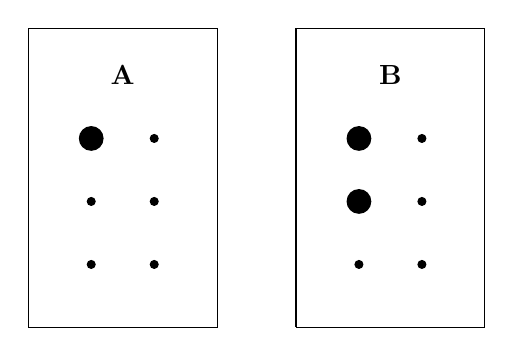
\begin{tikzpicture}
     \draw (0,0)--(2.4,0)--(2.4,3.8)--(0,3.8)--(0,0);
     \draw (3.4,0)--(5.8,0)--(5.8,3.8)--(3.4,3.8)--(3.4,0);
     \draw [fill](.8,.8) circle [radius=0.050];
     \draw [fill](.8,1.6) circle [radius=0.050];
     \draw [fill] (.8,2.4) circle [radius=0.150];
     \draw [fill](1.6,.8) circle [radius=0.050];
     \draw [fill](1.6,1.6) circle [radius=0.050];
     \draw [fill](1.6,2.4) circle [radius=0.050];
     \draw node at (1.2,3.2) {$\textbf{A}$};
     \draw [fill](4.2,.8) circle [radius=0.050];
     \draw [fill](5,.8) circle [radius=0.050]; 
     \draw [fill](4.2,1.6) circle [radius=0.150]; 
     \draw [fill](4.2,2.4) circle [radius=0.150];
     \draw [fill](5,1.6) circle [radius=0.050];
     \draw [fill](5,2.4) circle [radius=0.050]; 
    \draw node at (4.6,3.2) {$\textbf{B}$};
    \end{tikzpicture}
\end{center}
Qual o número máximo de caracteres distintos que podem ser representados neste sistema de escrita?
    \begin{enumerate}[(a)]
    \item 89
    \item 26
    \item 720
    \item 36
    \item 63
    \end{enumerate}
      \begin{sol}
        resposta: e \\
        $\frac{\phantom{A}}{2}\frac{\phantom{A}}{2}\frac{\phantom{A}}{2}\frac{\phantom{A}}{2}\frac{\phantom{A}}{2}\frac{\phantom{A}}{2}=2^6\Longrightarrow64-1=63$
      \end{sol}
\end{ex}